%\documentclass{emulateapj}
\documentclass[letterpaper,12pt,preprint]{aastex}

% packages
\usepackage{amssymb,amsmath,amsbsy}
\usepackage{booktabs}
\usepackage{bbold}
\usepackage{mathrsfs}
\usepackage{subfigure}
\usepackage[backref,breaklinks,colorlinks,citecolor=blue]{hyperref}
\usepackage[yyyymmdd]{datetime}
\renewcommand{\dateseparator}{-}

% commands
\newcommand{\given}{\,|\,}
\newcommand{\dd}{\mathrm{d}}
\newcommand{\transpose}[1]{{#1}^{\mathsf{T}}}
\newcommand{\inverse}[1]{{#1}^{-1}}
\newcommand{\msun}{\ensuremath{\mathrm{M}_\odot}}
\newcommand{\bs}[1]{\boldsymbol{#1}}
\newcommand{\ident}{\mathbb{1}}
\newcommand{\inttime}{t_{\rm int}}
\newcommand{\fdrate}{\mathcal{R}_\Omega}

\newcommand{\act}{J}
%\newcommand{\jac}{\bs{\rm J}}
%\newcommand{\jac}{\bs{G}}
\newcommand{\jac}{\mathscr{J}}

\begin{document}

\title{Chaotic diffusion of tidal streams}
\author{Adrian M. Price-Whelan\altaffilmark{\colum,\adrn},
	    Kathryn V. Johnston\altaffilmark{\colum},
	    Monica Valluri\altaffilmark{\mich},
	    Sarah Pearson\altaffilmark{\colum},
	    Andreas H. W. K\"upper\altaffilmark{\colum},
	    David W. Hogg\altaffilmark{\nyu,\cds,\mpia}}
\date{\centering \today}

% Affiliations
\newcommand{\colum}{1}
\newcommand{\adrn}{2}
\newcommand{\mich}{3}
\newcommand{\nyu}{4}
\newcommand{\cds}{5}
\newcommand{\mpia}{6}
\altaffiltext{\colum}{Department of Astronomy, 
		              Columbia University, 
		              550 W 120th St., 
		              New York, NY 10027, USA}
\altaffiltext{\adrn}{To whom correspondence should be addressed: adrn@astro.columbia.edu}
\altaffiltext{\mich}{Department of Astronomy, 
			   University of Michigan,
			   Ann Arbor, MI 48109, USA}
\altaffiltext{\nyu}{Center for Cosmology and Particle Physics,
                      Department of Physics, New York University,
                      4 Washington Place, New York, NY, 10003, USA}
\altaffiltext{\cds}{Center for Data Science,
                      New York University,
                      4 Washington Place, New York, NY, 10003, USA}
\altaffiltext{\mpia}{Max-Planck-Institut f\"ur Astronomie,
                     K\"onigstuhl 17, D-69117 Heidelberg, Germany}

\begin{abstract}

% Context
The large-scale, smooth components of galactic gravitational potentials are thought to be triaxial in shape.
Triaxial potentials that match observational constraints and measurements of the radial profile and axis ratios of dark matter halos in cosmological simulations are almost certainly not globally integrable. 
An appreciable number of chaotic orbits are therefore expected in galactic halos.
It is yet unclear whether chaotic regions of phase-space will affect the density evolution of stellar tidal streams, which form in the halos of galaxies from the disruption of stellar systems.
% Aims
Many numerical methods exist for assessing the degree of chaos for a given orbit (e.g., the Lyapunov exponent, the frequency diffusion rate). 
These indicators, which are local to a single orbit, often predict a timescale over which chaos will be dynamically important.
In this paper, we aim to compare these timescales to the density evolution of the finite-volume ensembles of orbits.
% Methods: 
We derp derp derp.
% Results:
We find that mean indicators such as the Lyapunov time or the (long term) frequency diffusion rate of a given ``parent'' orbit are not good predictors for the short-term density evolution of ensembles of orbits around this parent orbit.
Instead, we find that the variance of the fundamental frequencies of the ensemble orbits over short timescales is a stronger indicator of the density evolution.
% Conclusions:


\end{abstract}

\keywords{
}

\section{Introduction}\label{sec:introduction}

The dark matter halos of galaxies are thought to be triaxial in shape. Despite suggestive evidence from a range of complimentary observational methods, this fundamental prediction from $\Lambda$CDM cosmology has not been conclusively verified. Around other galaxies, it is generally hard to measure the 3D mass profile because they are seen in projection. From the Earth's position within the Milky Way, our view of our own halo and proximity gives us a unique chance to directly measure the 6D positions of stars and model the shape of the mass distribution at large radii. The Milky Way halo has a low density of visible tracers, but luckily many of the halo stars are likely on non-random orbits and thus contain extra information (e.g., debris stripped from in-falling satellite galaxies).

As a satellite galaxy or globular cluster orbits within some larger system, mass is eroded due to the tidal forces of the host galaxy potential. If the orbit of such an object is regular, only mildly eccentric, and stays far from sharp density features (e.g., the disk), the disruption is a steady process and the mass is slowly stretched into long streams of matter known as stellar tidal streams. The phase-space density and therefore the observable properties of these tidal streams are sensitive to the internal progenitor properties, orbit of the progenitor, and mass distribution of the host galaxy. Many tidal streams are observed around the Milky Way, M31, and other nearby galaxies (cite many). Around the Milky Way, streams are found over a large range of distances ($\approx$10-100~kpc). The morphological evolution of the debris depends on the spread of orbital properties (e.g., actions or frequencies) of the debris and the orbit of the progenitor system, both of which are also set by the shape and radial profile of the gravitational potential of the host galaxy. By simultaneously modeling the observed phase-space density of stream stars along with the potential, it is hoped that we may infer the dark matter distribution around the Milky Way.

Tidal streams are generally modeled as 1D structures formed on regular orbits with simple internal progenitor dynamics and density evolution. Methods span a range of complexity from orbit-fitting, to \emph{Streakline} or particle-spray models, to action-space density modeling, to N-body simulations \citep[see, e.g., the introduction of][]{kuepper15}. All methods have been tested in some way on simulated observations of data and these tests typically demonstrate the recovery of parameters for analytic, static potential forms. Many of the methods have been shown to work in axisymmetric or otherwise simple potentials but claim to extend to more complex, generalized potentials (e.g., triaxial or multi-component potentials). 

One example of stream modeling in a multi-component (static, analytic) potential was done by \citet{pearson15}, who tried to reproduce observations of the stellar stream density from the globular cluster Palomar 5 in a single oblate and single triaxial potential using \emph{Streakline} models \citep{kuepper12}. They use the observed SDSS number density of stars and a limited number of radial velocities measured for stream members to fit model streams to the data. In the oblate potential (a three-component bulge+disk+spherical halo potential), a thin model stream is easily found that reproduces the observed stellar density morphology of the stream. In the triaxial potential (the potential from \cite{law10}: a three component bulge+disk+triaxial halo fit to Sagittarius stream data), the model streams generically form large, two-dimensional ``fans'' of debris near the ends, and there are no physically reasonable progenitor orbits that reproduce the observed thinness of the stream given the observational constraints of the present-day position and velocity of the cluster. % In order to extend tidal stream models to more generic potentials, it is important to understand why this stream-fanning occurs and whether this and other strange debris morphologies are generic to more complex potentials. 

The obvious difference between the two potentials considered by \citet{pearson15} is the extra symmetry of the oblate potential. It is well known that the number of degrees of freedom of a potential plays a critical role in determining the orbit structure in the potential. Potentials (Hamiltonians) with more than two degrees of freedom generically contain significant chaotic regions. \citet{pearson15} tested the stochasticity of the orbit of the progenitor that produced fanned debris by computing the Lyapunov exponent but found that the orbit is consistent with being regular over dynamically relevant timescales (many Hubble times). It has been shown previously that along some strongly chaotic orbits, tidal streams form large, diffuse fans of debris \citep[e.g.,][]{fardal14}. However, it is unknown how the resultant properties of the debris (e.g., density or length of the stream) depend on the degree of stochasticity. The result from \citet{pearson15} suggests that even a weak chaos (as measured by the Lyapunov exponent) may affect the density evolution and therefore observability of tidal streams. 

TODO: this paragraph needs to be reworked...
In this work, we analyze whether the final configuration-space morphology of simple tidal stream models is correlated with measures of chaos local to the orbit of the progenitor. The effect of chaos in the halos of galaxies has largely been neglected because the chaotic timescales estimated were thought to be many times the age of the universe, but recent work has shown that even weak chaos may be relevant for tidal stream morphology. In this Article, we choose a simple, cosmologically motivated model for a triaxial potential, analyze the degree of chaos for grids of constant-energy orbits as computed from single-orbit diagnostics, and compare these results to measures of the mixing time of finite-volume ensembles of orbits (analogs to tidal debris). Finally, we connect the ensemble mixing rate to observational properties of streams, thus demonstrating that local orbital measures of chaos are predictors of tidal stream morphology. This provides a strong case for developing a method to use the mere existence of the many thin streams found in the halo of our own Galaxy to rule out classes or shapes of possible potentials that fit the Milky Way.

This paper is organized as follows: We review relevant nonlinear dynamics in Section~\ref{sec:nldreview}. In Section~\ref{sec:methods}, we describe our choice of potential and method for numerical orbit integration. We present our results in Section~\ref{sec:results} and discuss their implications in Section~\ref{sec:discussion}. We conclude in Section~\ref{sec:conclusions}.

% , we describe the connection between different measures of chaotic behavior, further discuss the implications of chaotic mixing, and comment on the applicability of the methods presented here to more realistic Galactic potentials and simulations.

%[Does this go anywhere?]
%Thin stellar streams form when the spreading of the debris is faster in some preferred direction \citep[one eigenvalue of the Hessian of the potential is large relative to others e.g.,][]{helmi99, sanders??}. This is generically the case for orbits with significant angular momentum in a spherical potential ($|L| > J_r$, orbits that we expect for form streams), but [... comments about expectations in more complex potentials] In a spherical or mildly axisymmetric potential, the debris can only really spread in a single dimension because somehow the constraint that .... Along chaotic orbits, Hessian not defined and frequencies diffuse, ...

\section{Review of nonlinear dynamics}\label{sec:nldreview}

% TODO: move all except chaotic diffusion stuff to appendix?

An orbit in an $N$ degree of freedom (dof) Hamiltonian, $H$, is a set of $2N$ quasi-periodic time series, 
\begin{equation}
(w_1(t),...,w_{2N}(t)) = (q_1(t),...,q_{N}(t),p_1(t),...,p_{N}(t)) \label{eq:coords}
\end{equation}
where $q_i$ and $p_i$ are conjugate coordinates in the sense that
\begin{align}
	\dot{p}_i &= -\frac{\partial H}{\partial q_i}\\
	\dot{q}_i &= \frac{\partial H}{\partial p_i}
\end{align}
for all $t$. The motion in any component, $w_i(t)$, can be represented as a Fourier sum,
\begin{equation}
	w_i(t) = \sum_k^\infty a_k \, e^{i\,\omega_k\,t}; \, (a_k \in \mathbb{C}). \label{eq:fourier}
\end{equation}

A \emph{regular orbit} is a set of such time series that can be transformed to a special set of canonical coordinates known as angle-action coordinates. In these coordinates, the position variables are angles, $\boldsymbol{\theta}$, that increase linearly with time with rates set by $N$ constant, fundamental frequencies, $\boldsymbol{\Omega} = (\Omega_1, ..., \Omega_N)$. The frequencies in the Fourier sum of any individual component of motion (the $\omega_k$ in Equation~1) are just linear, integer combinations of the fundamental frequencies, $\boldsymbol{\Omega}$ --- that is, for a regular orbit, any Fourier component frequency may be written
\begin{align}
	\omega_k &= \boldsymbol{n_k} \cdot \boldsymbol{\Omega}; \, (\boldsymbol{n}_k \in \mathbb{Z}^3). \label{eq:fourierfreq}
\end{align}
The conjugate momentum coordinates --- the actions,  $\boldsymbol{J}$ --- are constants of motion. Even stronger, the actions are isolating integrals and any pair are in involution such that
\begin{equation}
	[J_i, J_j] = 0
\end{equation}
where $[\cdot,\cdot]$ is the Poisson bracket. This implies that for an $N$ dof system, a regular orbit has $N$ independent constants of motion and the motion is therefore restricted to an $N$-dimensional manifold embedded in the 2$N$ dimensional phase space. The conjugate angle variables define an orthogonal basis, and the topology of angle-action space is therefore the product of $N$ circles, an $N$-torus. Any regular orbit in an $N$ dof Hamiltonian can be understood as motion on the surface of an $N$-torus. Each set of actions, $(J_1,...,J_N)$, uniquely labels a torus, and regular orbits may be referred to in terms of their orbital tori. If a transformation to angle-action variables exists, the Hamiltonian may be written solely in terms of the actions,
\begin{equation}
	H = H(\boldsymbol{J})
\end{equation}

A Hamiltonian or potential is said to be \emph{globally integrable} when the number of isolating integrals of motion is equal to the number of degrees of freedom and a transformation to angle-action coordinates may be done globally --- that is, the transformation to angle-action coordinates may be written as a function of arbitrary phase-space coordinates and the functional form is independent of phase-space position. The condition for global integrability is very restrictive and it seems that the likelihood that a Hamiltonian is globally integrable decreases as the number of degrees of freedom increase \citep[e.g.,][]{lichtenberg83}. 

Galactic potentials are almost certainly not globally integrable, but it is useful to understand the orbit structure in integrable systems before extending to more general potentials. Only one globally integrable triaxial mass model is known that generates motion that is qualitatively similar to that seen in Galaxies: the St\"ackel or ``Perfect Ellipsoid'' model \citep[e.g.,][]{kuzmin56, kuzmin73, deZeeuw85, cincotta06}. The four general classes of orbits in this potential are box, inner long-axis tube, outer long-axis tube, and short-axis tube orbits. Unlike the box orbits, the tube orbits preserve a sense of rotation about either the long or short axis.

Over long times, a generic orbit in this potential fills the surface of its 3-torus --- that is, the three fundamental frequencies of the orbit are incommensurable. If there exists a relation of the form
\begin{equation}
	\boldsymbol{n} \cdot \boldsymbol{\Omega} = n\, \Omega_1 + m\, \Omega_2 + l\, \Omega_3 = 0
\end{equation}
then the orbit is a resonant orbit and the effective dimensionality of the orbit is decreased to 2D. We refer to orbits that obey a single resonance relation as \emph{uni-resonant} orbits. If an additional resonance relation exists, the orbit is closed and becomes a 1D curve; we refer to such orbits as \emph{bi-resonant} orbits. The resonant structure of a potential --- the relative importance of particular resonance numbers --- is difficult to compute, but determines the global behavior of orbits in the potential. \cite{cincotta06} analytically compute the resonant structure in action-space for a St\"ackel potential. In frequency-space, the resonances are planes, but in action-space are generic 2D surfaces.

The orbit structure of non-integrable potentials can be qualitatively understood by considering a Hamiltonian that is a small perturbation away from being globally integrable --- that is, a Hamiltonian that may be written
\begin{equation}
	H(\boldsymbol{J}, \boldsymbol{\theta}) = H_0(\boldsymbol{J}) + \epsilon \, H_1(\boldsymbol{J}, \boldsymbol{\theta})
\end{equation}
where $\epsilon$ is a small parameter that determines the perturbation strength \citep[a complete description of perturbation theory applied to nonlinear Hamiltonians is given in][]{lichtenberg83}. When $0 < |\epsilon| \ll 1$, resonant surfaces become ``thick'' resonant layers, within which orbits are qualitatively similar to the parent resonant orbit \citep[e.g.,][]{merritt99} and the stable regions are surrounded by chaotic layers where stochastic motion occurs. Stochastic or chaotic orbits are characterized by apparently random behavior despite being generated by entirely deterministic systems. The stochastic layers form gaps in action space where tori are destroyed. The orbits that exist in these regions therefore can not be represented in angle-action coordinates, as their actions and frequencies evolve with time. 

Stochastic motion or the diffusion of an orbit in actions and frequencies may occur either \emph{across} the resonance layers or \emph{along} the stochastic layers (Arnold diffusion). For weakly chaotic orbits, motion across a resonance layer typically occurs with a frequency close to the libration frequency of the nearby stable orbits in the resonance layer. Thus, if the resonance libration frequency is comparable to the orbital frequency, motion across a resonance can modulate the frequency spectrum of an orbit over an orbital time. However, the stochastic layers are often bounded in the direction orthogonal to the resonance by other stable, resonant regions so that the frequencies or actions can't change by large factors (unless there is resonance overlap and the motion is strongly chaotic). The rate of diffusion along stochastic layers via Arnold diffusion depends on the local resonant structure and is hard to predict, however, this has been done analytically for simple potentials \citep[e.g.,][]{chirikov??}. For systems with $N>2$ dof, the stochastic layers connect and form an intricate network of stochasticity known as the Arnold web; the implication of this connectivity is that an orbit may dramatically change its appearance as it navigates through the Arnold web, though the timescales for this to occur are typically many 1000s of orbital periods.

When $\epsilon$ is large, there is no general prediction for the resulting behavior. It seems that more complicated and physically motivated triaxial potential models for galaxies follow the intuition gained from the small-perturbation picture described above, at least for certain parameter choices \citep{valluri, merritt, dehnen, etc.}. 

%For an integrable Hamiltonian, $H$, with $N$ degrees of freedom (dof), the equations of motion are most simply expressed in angle-action coordinates \cite[e.g.,][]{goldstein80}. In these coordinates, the actions, $J_n$, are (isolating) integrals of the motion, and the conjugate angle variables, $\theta_n$, increase linearly with time
%\begin{align}
%	\dot{\act}_n &= -\frac{\partial H}{\partial \theta_n} = 0\\
%	\act_n &= {\rm const.}\\
%	\dot{\theta}_n &= \frac{\partial H}{\partial \act_n} = \Omega_n(\act_1,\act_2,...,\act_n)\label{eq:aafreq}\\
%	\theta_n(t) &= \Omega_n t + \theta_n(0)
%\end{align}
%where $i=1,2,...N$, and $\Omega_n$ are the fundamental frequencies of the orbit.  The topology of angle-action space is equivalent to that of the surface of an $N$-dimensional torus, and thus orbits are often referred to in terms of \emph{orbital tori}: each set of actions, $(\act_1,\act_2,...\act_N)$, uniquely ``label'' the torus associated with a given orbit and the angles specify the location on the surface of the $N$-torus. If a global transformation to angle-action coordinates exists, the potential is said to be \emph{integrable}.
%
%Galactic gravitational potentials will almost certainly not be globally integrable. Dark matter halos of galaxies are expected to be triaxial but even if they are close to axisymmetric or spherical, the superposition of components (e.g., disk, bulge, halo) will break global integrability. If a triaxial (three dof) potential is close to integrable such that the Hamiltonian can be written in terms of a small perturbation, $\epsilon$, away from some integrable Hamiltonian, $H_0$,
%\begin{equation}
%	H(\bs{\theta}, \bs{\act}) = H_0(\bs{\act}) + \epsilon H_1(\bs{\theta}, \bs{\act})
%\end{equation}
%then a large number of regular orbits will survive the perturbation (by way of the KAM theorem)\footnote{3-vectors are represented with bold symbols, e.g., $\bs{J}=(J_1,J_2,J_3)$.}. The tori that survive will in general be separated by regions of irregular or chaotic motion, and thus any transformations to angle-action coordinates can only be defined locally. Analytic transformations to angle-action coordinates are only known for a handful of simple, integrable potentials. Much effort has gone in to developing general methods for transforming either from position-velocity to angle-action coordinates, $(\bs{x},\bs{v})\rightarrow(\bs{\theta},\bs{J})$ \citep{many}, or vice-versa, $(\bs{\theta},\bs{J})\rightarrow(\bs{x},\bs{v})$ \citep{many}.
%
%The types of motion generic to triaxial systems can be split into several sub-categories (summarized in Figure~\ref{fig:orbit-tree}). Regular motion can be classified by the number of resonance relations obeyed \citep[e.g.,][]{lichtenberg83}: \emph{conditionally periodic} orbits obey no resonance relations, \emph{uni-resonant} orbits obey a single relation of the form $\bs{m}\cdot\bs{\Omega}=0$, and \emph{bi-resonant} orbits obey two resonance relations, $\bs{m}\cdot\bs{\Omega}=0$ and $\bs{n}\cdot\bs{\Omega}=0$, where $\bs{m}$ and $\bs{n}$ are integer vectors.
%
%% Figure 2
%%\begin{figure*}[!h]
%%\begin{center}
%%\includegraphics[width=0.6\textwidth]{figures/orbit-tree.pdf}
%%\caption{A rough classification of the types of orbits found in triaxial potentials. Regular orbits are classified by the number of resonance relations obeyed: conditionally periodic (\emph{none}), uni-resonant (\emph{one}), bi-resonant (\emph{two}). Irregular or chaotic orbits are simply separated into two classes: strongly and weakly chaotic, defined by the timescales of interest in a problem. When the characteristic chaotic timescale is much longer than, for example, the age of the universe, the orbit is only weakly chaotic. } \label{fig:orbit-tree}
%%\end{center}
%%\end{figure*}
%
%Truly resonant orbits are rare \citep{merritt99}, but dynamically important in systems with several degrees of freedom as they determine the structure of orbit-space. Stable, resonant orbits generate families of orbits that may behave or appear similarly, whereas unstable resonances are typically associated with regions of chaos. Not all orbits can be trivially associated with resonances due to the infinitely complex, hierarchical structure of resonances (though the importance or ``size'' of a resonance falls off inversely with the norm of its integer vector, $|\bs{m}|^{-\alpha}$, with $\alpha > 0$). In autonomous, two dof systems, stochastic regions are generally surrounded and separated by regular motion, thus chaotic orbits are confined. In three or more dof the chaotic regions will connect and overlap. This is the origin of Arnold diffusion \citep{arnold64}, which allows chaotic orbits to radically change shape by traversing the web of unstable resonances and are only strictly bounded to their own energy hypersurface. This phenomenon is perhaps easier to visualize in action-space: in two dof systems, if a given set of tori are destroyed due to potential perturbations, an orbit in this now chaotic region is still bounded between the surrounding tori due to energy conservation. In three dimensions, the extra degree of freedom allows chaotic orbits to ``escape'' this confinement.
%
%For small potential perturbations, many regular orbits survive and only small chaotic islands are introduced. As the strength of the perturbation increases, eventually all tori associated with conditionally-periodic motion will be destroyed. Next, the uni-resonant tori are destroyed, and finally the bi-resonant tori --- these are least susceptible to destruction from perturbations \citep[e.g., see][]{valluri98}. However, even orbits that are strictly chaotic may behave regularly over timescales much longer than, for example, the dynamical time of the system. Chaotic orbits can therefore be loosely classified by being either \emph{strongly} or \emph{weakly} chaotic: strongly chaotic orbits behave irregularly over a few ($\sim$10) dynamical times, whereas weakly chaotic orbits behave regularly over this timescale. This rough classification is tied to local measures, such as the Lyapunov time (Section~\ref{sec:lyap}) or frequency diffusion time (Section~\ref{sec:naff}). 
%
%These local measures quantify the divergence of infinitesimally nearby orbits or the rate of frequency diffusion along an orbit. For an ensemble of orbits with finite spreads in energy or frequencies (e.g., tidal debris), each orbit will have a slightly different characteristic timescale, but we still expect mixing time of the ensemble to correlate with local measures of chaos of the ``parent'' orbit of the ensemble (Section~\ref{sec:ensemble}). The evolution of tidal debris will depend on the ensemble mixing rate around the parent orbit: chaotic mixing will cause the density of the debris to fall off more quickly than the typical power-law behavior expected for regular orbits \citep[e.g.,][]{merritt96, helmi99}. 
%

\section{Numerical methods}\label{sec:methods}

\subsection{Potential choice}\label{sec:potential}

The density distributions within dark matter halos formed in cosmological N-body simulations are generically triaxial \citep[e.g.,][]{jing02, bett07, zemp09, veraciro11}. With the inclusion of baryonic physics and sub-grid prescriptions for energy input due to supernovae and other feedback mechanisms, the inner potential ($\lesssim$$0.1R_{\rm vir}$ for a $\approx$$10^{12}~\msun$ halo mass) typically becomes more spherical, though the magnitude of this reshaping depends on the particular merger history and star formation efficiency within a given halo \citep[e.g.,][]{dubinski??, recent NiHao stuff}. It is less clear what happens to the outer halo where tidal streams are more readily found. %; for this reason, we ask what we would expect to happen to tidal streams if the halo in which they form is strongly triaxial.

 \citet[][hereafter JS02]{jing02} found that a triaxial generalization of the classic NFW density profile \citep{navarro96} generates excellent fits to the density distributions within haloes in their high-resolution N-body simulations, and they provide probability distributions for the axis ratios of a large sample of these halos. JS02 finds median axis ratios of $c/a \approx 0.55$ and $b/a \approx 0.77$ where $a$ is the major axis, $b$ the intermediate, and $c$ the minor axis.\footnote{Note that JS02 use the opposite notation so that $c$ is the major and $a$ is the minor axis.} These are largely consistent with findings from more recent simulations \citep[e.g.,][]{??, NiHao} and consistent with constraints from weak lensing that place a lower limit on minor-to-major axis ratios of $c/a\gtrsim0.5$ \citep{vanuitert12}. JS02 finds significant scatter in the distributions of concentration parameter, $c_e$, or scale radius (depending on choice of parametrization). 

All of these parameters are specified in terms of the \emph{density}; for orbit analysis, we need to determine the form of the potential in terms of these parameters, which, in general, requires numerical integration of the density at each position of interest. For computational efficiency, many authors instead express the triaxiality in the form of the potential, but this can lead to unphysical situations where the density becomes negative. \citet{leesuto03} derive a perturbative expansion of the potential integral for a triaxial NFW density and show that the expansion is accurate even for modest axis ratios (e.g., the median values shown above). 

In this work, we use the triaxial potential expression from \citet{leesuto03}, parametrized in a slightly different manner. In terms of spherical coordinates\footnote{$(r,\phi,\theta)$ = (radius, azimuth, colatitude)} with the radius normalized by the scale radius, $u = r/r_s$
\begin{align}
	\Phi(u,\phi,\theta) &\approx \frac{v_c^2}{A}\left[F_1(u) + \frac{1}{2}(e_b^2 + e_c^2)F_2(u) + \frac{1}{2} [(e_b\sin\theta \sin\phi)^2 + (e_c\cos\theta)^2] F_3(u) \right]\\
	A &= \left(\ln2 - \frac{1}{2}\right) + \left(\ln2-\frac{3}{4}\right) (e_b^2 + e_c^2)
\end{align}
where $e_b = \sqrt{1 - (b/a)^2}$, $e_c = \sqrt{1 - (c/a)^2}$, and $v_c$ is the circular velocity at the scale radius, $r_s$, for the spherical case. The functions $F_i(u)$ are given in the appendix of \cite{leesuto03}. We chose $r_s=20~{\rm kpc}$ and $v_c = 175~{\rm km}~{\rm s}^{-1}$ by taking the mean halo concentration for a ${\rm M}_{vir} \approx 10^{12}~\msun$ halo, $c_e\approx5$, from \cite{jing02} and by assuming $R_{vir}\approx200~{\rm kpc}$. Figure~\ref{fig:potential} shows equipotential contours of this potential in projection.

This potential is a simple and unrealistic model for the total potential of a Milky-Way-like galaxy, however it represents a conservative choice for exploring the structure of orbits in the halos of such galaxies. Realistic Galactic potentials will have a significant component due to the disk and bulge, may have twisting inertia tensors (cite), radially changing axis ratios \citep[e.g.,][]{kazantzidis04,debattista08,veraciro11, NiHao}, significant substructure \citep{moore98,zemp09}, or time dependence \citep[either from bulk rotation, mass growth, mergers, etc.][]{bailin05}. We expect inclusion of any of these effects to increase the amount and influence of chaos; see the Discussion (Section~\ref{sec:discussion}) for a few simple demonstrations.

\subsection{Orbit integration}\label{sec:integration}

We use the Dormand-Prince 8th-order Runge-Kutta scheme \citep{prince81} to integrate orbits in the above potential. Specifically, we use a \texttt{Python} wrapper over the \texttt{C} implementation by \cite{hairer93}. For all orbits we ensure that energy is conserved to $\Delta E/E_0 \leq 10^{-8}$ by the end of integration, however most orbits conserve energy to $\Delta E/E_0 \approx 10^{-13}$. Unless otherwise specified the integration timesteps are chosen so that there are 512 steps per strongest orbital period component, but the integrator uses adaptive stepping between each main step in order to satisfy a specified tolerance (we set the absolute tolerance to $\approx$100 times machine precision, $\texttt{atol} = 10^{-13}$). 

\subsection{Lyapunov exponents} \label{sec:lyap}

The most well-known method for assessing chaotic motion is to analyze the Lyapunov spectrum or maximum Lyapunov exponent (MLE) of an orbit. The MLE measures the mean rate of divergence of two infinitesimally separated orbits and is only strictly defined in terms of a limit that goes to infinite time. Thus, we can never truly compute the MLE and it can take integration for many thousands of orbital periods to compute a converged numerical approximation of the MLE for a moderately chaotic orbit. In this work, we use the algorithm introduced by \cite{wolf85} for computing the MLE (for more a more detailed description of this algorithm, see Appendix~\ref{sec:lyapapdx}).

The MLE, $\lambda_{\rm max}$, is interpreted as a rate that determines the nature of exponential divergence of infinitesimally close chaotic orbits. It is therefore useful to consider the corresponding $e$-folding time, 
\begin{equation}
	t_{\rm \lambda} = \frac{1}{\lambda_{\rm max}}.
\end{equation}
We will use this as the prediction from the Lyapunov exponent for the timescale over which chaos should be dynamically important for a given orbit. 

\subsection{Numerical approximation of fundamental frequencies}\label{sec:naff}

Bounded, regular orbits in a triaxial potential will have three fundamental frequencies, $\bs{\Omega}$, that determine the periodic behavior of motion. The motion in any canonical coordinate can therefore be decomposed as a Fourier sum (Equation~\ref{eq:fourier}) where the Fourier frequencies are linear, integer combinations of the fundamental frequencies (Equation~\ref{eq:fourierfreq}). \cite{laskar93} introduced a method for recovering the fundamental frequencies of an orbit that effectively uses a Hamming-filtered fast-Fourier transform (FFT) of complex combinations of the motion (e.g., $x(t) + i v_x(t)$). It has been shown that using a filter makes the accuracy in determining the frequencies converge much faster than the typical $\inttime^{-1}$ expected for a standard FFT \citep{laskar99}, where $\inttime$ is the integration time. Once the strongest frequencies of the time series are found, the spectrum must be searched for the three fundamental frequencies.

This method is referred to as ``Numerical Approximation of Fundamental Frequencies'' (NAFF) and has been used extensively in planetary dynamics \citep{} and galaxy dynamics \citep{valluri98}, especially in the study of orbits in triaxial systems. We have implemented and tested our own open-source implementation of NAFF in \texttt{Python}.\footnote{This code is publicly available through the \texttt{Gary} package, \url{http://...}} Though our implementation differs slightly from the original definition and from that used in \cite{valluri98}, we still refer to the method as NAFF. For more details about NAFF, see Appendix~\ref{sec:naffapdx} or \cite{papaphilippou96, laskar, etc.}.

If an orbit is chaotic, the motion can no longer be expressed in terms of a single set of fundamental frequencies because the actions and frequencies of the orbit change with time. For a weakly chaotic orbit, the orbit may appear consistently periodic over long windows of time. NAFF will pick out a set of frequencies for such orbits that correspond to the largest peaks in the power spectrum of the stochastic orbits, however these peaks will change character with time. For more strongly chaotic orbits, the power spectrum will be quite noisy and the peak frequencies may change erratically when comparing two separate sections of orbit. The frequencies picked out by NAFF for such orbits will therefore represent the average periodic nature of the orbit over a given period. We define the fractional frequency diffusion rate per orbit, $\fdrate$, as
\begin{equation}
	\fdrate = \max_{\bs{a}} \, \left(\frac{\bs{\Omega}_{T_2} - \bs{\Omega}_{T_1}}{\bs{\Omega}_{T_1}}\right) \times \frac{1}{N_T}\label{eq:fdrate}
\end{equation}
where $\bs{\Omega}_{T_1}$ and $\bs{\Omega}_{T_2}$ are the fundamental frequencies computed from two consecutive sections of orbit, $N_T$ is the number of orbital periods within a single section of orbit computed from the most significant fundamental frequency, and the maximum is taken with respect to the corresponding amplitudes, $\bs{a}$, of the fundamental frequency components. The frequency diffusion rate as defined above (e.g., measured in the frequency with the largest amplitude) is better correlated with the strength of chaos in an orbit \citep{valluri??} but differs from the original definition of \cite{valluri98}.

From this rate, we can compute a timescale for the diffusion of the fundamental frequencies of an orbit. For a small ensemble of orbits, the relevant timescale is the time over which the change in frequencies for a single orbit is comparable to the spread of frequencies in the ensemble. We therefore define the frequency diffusion time with an unspecified parameter, $f$,
\begin{equation}
	t_\Omega = \frac{2 \pi}{\bs{\Omega}_{T_1}} \frac{f}{\fdrate}.
\end{equation}
When $f = 1$, this is the timescale over which we expect order-unity changes to the frequencies, whereas $f = 0.01$ corresponds to $1\%$ changes.

% =====================================================================
%	Results
%
\section{Results}

In previous work, we found that tidal debris from a simulated globular cluster (Palomar 5) on an orbit with a long Lyapunov time can form large ``fans'' of debris similar to those seen for progenitor systems on strongly chaotic orbits \citep{pearson15, fardal14}. Here, to illustrate the methods described above, we repeat the calculation of the Lyapunov exponent for the Pal 5, stream-fanning orbit of \cite{pearson15} with a longer integration time and compute the frequency diffusion rate. From these, we measure the Lyapunov time and frequency diffusion time. 

Figure~\ref{fig:pal5} shows the finite-time Lyapunov exponent computed for the Pal 5 orbit --- shaded region shows the ``converged'' part of the estimate that is used to compute the maximum Lyapunov exponent. By inverting the rate, we find $t_\lambda = XX~{\rm Gyr}$, consistent with our finding in \cite{pearson15}. We then compute the frequency diffusion rate (Equation~\ref{eq:fdrate}) using two consecutive integration windows with length $\approx$50 orbital periods. We find $\fdrate = 10^{-XX}$, which corresponds to a frequency diffusion time, $t_\Omega = XX~{\rm Gyr}$. Though this orbit is computed in a different potential than will be used below, this demonstrates the apparent discrepancy between the timescales over which chaos is estimated to be relevant (XX's of Gyrs) and the integration time over which stream-fanning becomes apparent ($<8$ Gyr). Below, we [...] try to understand by looking at grids of orbits...

\subsection{Part I: Lyapunov and frequency diffusion times}\label{sec:results1}

We generate isoenergy grids of initial conditions along the $xz$ ($y=0$) plane\footnote{$x$ is the major and $z$ the minor axis.} with energy (per unit mass) chosen to span a range of distances comparable to the scale radius of the potential (Section~\ref{sec:potential}), $E=-(397.2~{\rm km~s}^{-1})^2$ (in physical units). We fix $v_x = v_z = 0$, and compute $v_y$ from the energy. The majority of the orbits generated on this grid are tube orbits, which preserve a sense of rotation about one of the principal axes of the potential and are generally centrophobic. Tube orbits are generally less stochastic than box orbits --- the other major class of orbits in triaxial potentials --- which tend to plunge deep into the inner regions of the potential, however there are appreciable regions of stochastic tube orbits. Thin tidal streams are thought to form along tube orbits rather than box orbits because of the fast disruption expected for stellar systems on radially plunging orbits. The major classes of stable tube orbits circulate about either the major or minor axis. The most prominent orbits in this grid are the short-axis and outer long-axis tubes, but this grid generates all of the major orbit classes: short-axis tubes, long-axis inner tubes, long-axis outer tubes, stochastic intermediate-axis, and box orbits. 

To compute the Lyapunov exponents, we integrate all orbits in the grid for 1000 orbital periods and use the method described in Section~\ref{sec:lyap}. Figure~\ref{fig:lyapmap} shows the grid of initial conditions (in the $xz$ plane) --- each pixel corresponds to an orbit, and the logarithm of the Lyapunov time (in units of Gyr) is mapped to greyscale intensity. The darker pixels have shorter Lyapunov times and are more chaotic. By numerically estimating the MLE over this fixed integration window, the majority of orbits appear to be regular because they have exceedingly long Lyapunov times. 

For each orbit, we also separately integrate for $\approx$100 orbital periods and use NAFF to compute the fundamental frequencies for the two consecutive sections of 50 orbital periods. Figure~\ref{fig:freqdiff} shows the same grid of initial conditions, but now the greyscale intensity is set by the logarithm of the frequency diffusion time. The darker pixels have shorter frequency diffusion times and are more chaotic. This map reveals the intersection of this particular energy hypersurface with the rich structure of resonant surfaces present in this potential. This map highlights the accuracy of NAFF --- weak chaos is detected over $\approx$100 orbital periods, compared to the many thousands of orbits it would take to detect such features with the maximum Lyapunov exponent. The tube orbits in this potential are mostly regular or only mildly chaotic --- the largest regular regions are associated with the short-axis and long-axis tube orbits --- however islands of stronger chaos do appear, especially at the intersections of resonances where resonance overlap occurs. 

The strongest chaotic regions appear in both of the above grids (Figure~\ref{fig:lyapmap} and Figure~\ref{fig:freqdiff}), but the timescales [...]. Figure~\ref{fig:lyapvfreqdiff} shows the Lyapunov time plotted against the frequency diffusion time [...]. frequency diffusion rate is more accurate and thus more sensitive to mild chaos. It is unclear whether these regions will be dynamically important on realistic timescales, but we have confirmed from two independent methods that there are regions of strongly chaotic orbits even in this simple, triaxial potential.

The frequency diffusion time grid reveals the intricate resonant structure of the potential considered, but the majority of the orbits have predicted chaotic timescales that correspond to many hundreds or thousands of orbital times. In the next section, we compute the mixing rates for finite-volume ensembles of orbits and compare the density evolution of the ensembles to the predictions from the single-orbit chaos diagnostics of this section.

\subsection{Part II: Ensemble properties and mixing} \label{sec:results2}

The Lyapunov time and frequency diffusion rate measure the timescales over which chaos is relevant \emph{local} to a given orbit --- that is, these quantities are measures of how infinitesimal deviations will diverge, on average, from some parent orbit of interest. Tidal debris is disrupted from progenitor systems with finite spreads in orbital properties (e.g., energy). For a disrupting, globular-cluster-scale progenitor, the typical energy dispersion of the debris is 0.1--1\% of the progenitor orbital energy, but for a dwarf-galaxy-scale progenitor, the dispersion can be 5--20\%. This raises an important consideration: do finite deviations diverge faster than predicted from local measures of chaos? Does the Lyapunov or frequency diffusion time predict the timescale over which a finite phase-space volume (e.g., tidal debris) stays ``coherent''?

We start by considering three particular orbits chosen from the orbit grid of Section~\ref{sec:results1}: a regular orbit (R), a weakly chaotic orbit (W), and a strongly chaotic orbit (S). The orbits were chosen at random from a single column of the orbit grid based on their frequency diffusion time, and the initial conditions and chaos diagnostics are listed in Table~\ref{tbl:three-orbits}. We use the Self-Consistent Field (SCF) basis function expansion code \citep{hernquist92} to run N-body simulations of tidal stream formation from globular-cluster-mass progenitor systems on these three orbits. [TODO: mass scale 2.5E4 and mass contained within??] For each simulation, the progenitor consists of a $10^4$ particle Plummer sphere and the background triaxial NFW potential is turned on slowly over 250 Myr to reduce artificial gravitational shocking. We start the progenitor systems at apocenter and evolve for $\approx$16 orbital periods so that each simulation finishes again at subsequent apocenter. Figure~\ref{fig:nbodysims} shows the final particle distributions rotated so that the angular momentum of the progenitor orbit is aligned with the $z$-axis. A thin, cold stream forms on the regular orbit, a more diffuse stream on the mildly chaotic orbit, and a ``fanned'' stream on the strongly chaotic orbit. Given the long Lyapunov and frequency diffusion times of the mildly chaotic orbit, it is surprising that stream formed on this orbit appears to be more diffuse than the regular orbit stream. 

\begin{table*}[ht]
\begin{center}
	\begin{tabular}{c | c c c c c c | c c }
		{\bf ID} & $\bs{x}$ & $\bs{y}$ & $\bs{z}$ & $\bs{v_x}$ & $\bs{v_y}$ & $\bs{v_z}$ & $\bs{t_\lambda}$ & $\bs{t_\Omega}$ \\\toprule
		R & 27.30 & 0 & 1.10 & 0 & 183.61 & 0 & XX & YY\\
		\midrule
		W & 27.30 & 0 & 20.30 & 0 & 121.20 & 0 & XX & YY\\
		\midrule
		S & 27.30 & 0 & 21.90 & 0 & 111.22 & 0 & XX & YY\\
		\bottomrule
		\end{tabular}
	\caption{Orbits from the $xz$ grid with a range of chaotic timescales --- R is a regular orbit, W a weakly chaotic orbit, and S a strongly chaotic orbit. Positions ($x$, $y$, $z$) are given in kpc, velocities ($v_x$, $v_y$, $v_z$) in km~s$^{-1}$, and times ($t_\lambda$, $t_\Omega$) in Gyr. \label{tbl:three-orbits}}
\end{center}
\end{table*}

It is computationally intractable to run full N-body simulations for the large grid of orbital initial conditions used for the maps of the previous section and we therefore take a simplified approach for studying how finite-volume debris spreads along each of these orbits. We instead consider small ensembles of particles meant to represent debris disrupted from a single tidal disruption event. For a given set of orbital initial conditions --- the ``parent'' orbit --- we find the position of the nearest pericenter, initialize a small ensemble of test particle orbits around this position, then follow the orbits of all test particles for an integration time equal to XXX times the longest fundamental orbital period. The physical scale of the ensemble is set by the tidal radius in position and velocity scale in velocity and are therefore set by the mass scale of the progenitor \citep[e.g.,][]{johnston98, apw14}. If $(\bs{x}_0,\bs{v}_0)$ are the parent orbit initial conditions at pericenter, then $(\delta\bs{x}_i,\delta\bs{v}_i)$ is the deviation vector of the $i$th particle and the magnitude of the offsets are assumed to be Normally distributed away from the parent orbit:
\begin{align}
	\delta\bs{x}_i &\sim \mathcal{N}(0, r_{\rm tide})\\
	\delta\bs{v}_i &\sim \mathcal{N}(0, \sigma_v)\\
	r_{\rm tide} &= \|\bs{x}_0\| \left(\frac{m}{3M_{\rm enc}(\|\bs{x}_0\|)}\right)^{1/3} \\
	\sigma_v &= \|\bs{v}_0\|\left(\frac{m}{3M_{\rm enc}(\|\bs{x}_0\|)}\right)^{1/3} 
\end{align}
where $M_{\rm enc}(r)$ is the mass enclosed of the host potential within radius $r$, $m$ is the mass scale of the debris, and $\|\cdot \|$ is the Euclidean norm. We take $m=10^4~\msun$ to represent globular-cluster-like progenitors, and use the spherically-averaged enclosed mass of the host potential to estimate the above debris scales.




Over long times, a chaotic orbit will ergodically mix over the surface of its energy hypersurface (dimensionality 5 in a triaxial potential) whereas a (non-resonant) regular orbit will mix over the surface of its 3-torus.

 We instead use ensembles with small spreads in energy so that we expect that most ensemble particle orbits around a parent chaotic orbit will reach a fully mixed state but now the final distribution will have some thickness around this surface. Around a typical regular orbit, each individual orbit will fill its torus ergodically --- a surface with lower dimension than the energy hypersurface --- and thus, a small enough ensemble should never reach the fully mixed state as defined above because it will remain confined to a subspace of lower dimensionality.


[TODO: wait, actually, they differ in a log -- why doesn't this change things more? I guess this is saying like, mean(log(dens)) ~ log(mean(dens))??? confuzzled]
As the particle ensembles evolve in time, we follow the mean configuration-space density of each to quantify the degree of mixing of the ensembles. This is similar to the method of \citet{merritt96} who measured the evolution of the relative entropy between the configuration-space density of isoenergy ensembles, $\rho(\bs{x},t)$, and the density of an ensemble that is uniformly distributed over the energy hypersurface, $\rho_{E_0}(\bs{x})$. In our case, the

 [but isoenergy so constant...yadda yadda].

to quantify the degree of mixing of the ensemble by computing the ``distance'' between the configuration space density of the ensemble at a given time, $\rho(\bs{x},t)$, with that of a distribution that is uniformly distributed over the energy hypersurface, $\rho_{E_0}(\bs{x})$, where $E_0$ is the energy of the parent orbit and thus hypersurface of interest. Our method differs in a few ways from that of MV96. First, MV96 use isoenergy ensembles of particles for following the density because this is the only way to guarantee that, if chaotic, nearly all orbits in the ensemble will lie on chaotic orbits. We instead use ensembles with small but finite spreads in energy; we still expect that most ensemble particle orbits around a parent chaotic orbit will reach a fully mixed state but now the final distribution will have some thickness around this surface. Around a typical regular orbit, each individual orbit will fill its torus ergodically --- a surface with lower dimension than the energy hypersurface --- and thus, a small enough ensemble should never reach the fully mixed state as defined above because it will remain confined to a subspace of lower dimensionality. In practice, only strongly chaotic systems will get close to $\rho_{E_0}(\bs{x})$ in a reasonable amount of time; we expect the rate to depend on how stochastic the parent orbit is (e.g., as measured by the Lyapunov time or frequency diffusion rate) and also on how ``trapped'' the chaotic region is (a small chaotic region wedged between stable tori will take longer to appear chaotic, even if internally the frequency diffusion rate is large). However, the difference in configuration space density between an ensemble undergoing chaotic mixing versus an ensemble around a regular orbit may be detectable over a much shorter timescale. The fully-mixed, normalized, configuration-space density that fills a given energy hypersurface, $E_0$, is easily found by projecting the simple distribution function, $f$, into configuration space:
\begin{align}
	f(\bs{x}, \bs{v}) &= f_0 \, \delta(H(\bs{x}, \bs{v}) - E_0)\\
	\rho_{E_0}(\bs{x}) &= \int \dd^3v \, f(\bs{x}, \bs{v})\\
	&= \int \dd^3v \, f_0 \, \delta(H - E_0)\\
	&= 4\pi \int \dd v \, v^2 \, f_0 \, \delta\left(v^2/2 + \Phi(\bs{x}) - E_0\right)\\
	&= A \sqrt{E_0 - \Phi(\bs{x})}\label{eq:mixeddensity}
\end{align}
where $A$ is a constant determined such that $\int \dd^3\bs{x} \, \rho_{E_0}(\bs{x}) = 1$, and $\delta(\cdot)$ is the Dirac delta function. 

For each ensemble, we compute the Kullback-Leibler divergence \citep[KL divergence;][]{kullback51} between the configuration-space density and the fully-mixed density (Equation~\ref{eq:mixeddensity}) by estimating the configuration space density $\rho(\bs{x},t_j)$ using kernel density estimation (KDE)\footnote{We use an implementation from the Python package scikit-learn \citep{scikitlearn}.} with the ensemble of particle positions at a given time $t_j$, We use Monte Carlo integration to evaluate the KL divergence rather than evaluate the integral over a three dimensional grid. The KL divergence, $D_{\rm KL}$, is a measure of the relative (Shannon) entropy between two normalized density functions, $p(x)$ and $q(x)$,
\begin{equation}
	D_{\rm KL} = \int \dd x \, p(x) \ln \frac{p(x)}{q(x)}
\end{equation}
Instead, we are computing the three dimensional integral
\begin{align}
	D_{\rm KL}(t_j) &= \int \dd^3 \bs{x} \, \rho(\bs{x},t_j) \ln \frac{\rho(\bs{x},t_j)}{\rho_{E_0}(\bs{x})}
\end{align}
where we only have an estimate of the density $\rho_{\rm KDE}(\bs{x},t_j) \approx \rho(\bs{x},t_j)$. Using samples from this KDE estimated density, $\bs{x}_i$, the KL divergence is
\begin{align}
	D_{\rm KL}(t_j) &\approx \frac{1}{N} \sum_i^N \ln \frac{\rho_{\rm KDE}(\bs{x}_i,t_j)}{\rho_{E_0}(\bs{x}_i)}\\
	\bs{x}_i &\sim \rho_{\rm KDE}(\bs{x},t_j)\label{eq:sampled_from}
\end{align}
where Equation~\ref{eq:sampled_from} indicates that the $\bs{x}_i$ are samples from the KDE density. For any computation of the density estimate, we use 10-fold cross-validation to find the optimal kernel bandwidth, $\sigma_{\rm KDE}$, by maximizing the likelihood of withheld particles.

Figure~\ref{fig:DKL} shows $D_{\rm KL}$ as a function of time for the two orbits of Section~\ref{sec:comparison}. The chaotic orbit (Orbit B, dashed line) ensemble mixes much faster than the regular orbit (Orbit A, solid line) ensemble. The KLD is related to the logarithm of the mean density of the debris so that a difference of 1 in the KLD roughly corresponds to a factor of 10 difference in mean density of the debris. Figure XX shows particle positions at apocenter after 2, 16, and 32 orbital periods of evolution for ensembles of 1000 particles generated around Orbit A and B. For visualization, the final positions are rotated to lie on the $x$ axis and the angular momentum vector of the parent orbit at the given time is aligned with the $z$ axis.

From the decay of the KLD, we measure a mixing rate by [TODO: how?].

Our goal is to characterize the morphology of tidal debris along orbits generic to triaxial potentials. For example, it has been shown that along some chaotic orbits, tidal streams form large, diffuse ``fans'' of debris \citep[e.g.][]{fardal14, pearson15}, however, it is unknown how the observable properties of the debris (e.g., density or length of the stream) depend on the degree of stochasticity. Further, quantifying the degree of stochasticity with, for example, the frequency diffusion rate represents a \emph{local} measure of chaos and it is unclear how this generalizes to the small but finite spreads in orbital characteristics common to debris that is tidally disrupted from globular clusters or dwarf satellite galaxies. To answer this question would require a massive exploration of parameter space --- both in potential and in orbits --- and thus would require a prohibitive number of N-body simulations to truly analyze the disruption process in all situations.

We measure the state of mixing of debris along the same grid of initial conditions as described above by computing the KL divergence (KLD) between the configuration-space density of the ensemble and the configuration-space density expected if the ensemble particles were uniformly distributed over the parent orbit energy hypersurface (Section~\ref{sec:ensemble}). From the time evolution of the KLD for a given ensemble around an orbit from the orbit grid, we estimate the mixing rate [TODO]. Figure~\ref{fig:kldmap} shows the same grids of initial conditions as plotted in Figures~\ref{fig:lyapmap} and \ref{fig:freqmap}, but now the intensity of the pixels is set by the [TODO].

\subsection{Part III: Short-time frequency evolution}\label{sec:results3}

Both the Lyapunov exponent and the frequency diffusion rate measure mean, long-term rates of chaotic diffusion. As discussed in Section~\ref{sec:nldreview}, frequency diffusion may occur either across a resonance layer or along a stochastic layer. If a weakly chaotic orbit is confined (by other nearby, non-overlapping resonances or stable regions), the mean drift of an orbit in frequency space will be small if computed over timescales long compared to the orbital time but short compared to the Arnold diffusion time. For the potential considered in this paper, these are precisely the timescales for which the frequency diffusion rate of the previous section were computed ($\sim$100's of orbital periods). This window length was chosen in order to have a strong enough signal in the frequency spectrum of chaotic orbits to measure the most significant frequencies using NAFF. 

In this section, we instead wish to resolve the short-time behavior of the frequency diffusion (corresponding to motion across resonance layers). For each orbit, we now instead use a rolling window to analyze the evolution of the frequency spectrum on shorter times. We use a window with a width of 50 orbital periods and shift the window by half an orbital period between each calculation of the most significant frequencies. [Why this window width? Stride?]

%\begin{figure}[!h]
%\centering
%	\includegraphics[width=0.4\columnwidth] {figures/kld-map.png}
%	\caption{Not the final figures. Need to re-make with same axis limits, remove labels, put in same PDF file...etc.} 
%	\label{fig:kldmap}
%\end{figure}

\section{Discussion}\label{sec:discussion}

We have shown that local measures of chaos [...]

Since all known tidal streams have been discovered as kinematic overdensities of stars, this implies (1) [something about accretion history], (2) the long, thin tidal streams we see may represent a sampling from ``special'' orbits in the Galactic potential where the mixing time is long, and (3) previous assumptions that connect the length and size of streams to their evolution time may be invalid.

Recovering the potential of triaxial systems is not trivial. Danger of orbit fitting because chaotic orbits can reproduce morphologies of regular orbits.

\subsection{Potential}

Why not disk + bulge? What do we expect when we add?

Real disk will be self-consistent with halo, so this isn't really a fair test, but still...

Other effects: radial dependence of axis ratios, time dependence, etc.

Moved from intro:
This also has implications for modeling the accretion histories of galaxies. Debris morphology is often separated into two classes --- streams (usually from high angular momentum progenitor orbits) and shells (from radially plunging orbits) --- but in practice the distinction may not be as clear due to other mixing effects.

\section{Conclusions}\label{sec:conclusions}
We have shown that ...

\acknowledgements
The authors wish to thank ... Robyn Sanderson, David Hogg, Dan D'Orazio, David Merritt, and the \emph{Stream Team} for useful comments and discussion.
APW is supported by a National Science Foundation Graduate Research Fellowship under Grant No.\ 11-44155. 
This research made use of Astropy, a community-developed core \texttt{Python} package for Astronomy \citep{astropy13}.
This work additionally relied on Columbia University's \emph{Hotfoot} and \emph{Yeti} compute clusters, and we acknowledge the Columbia HPC support staff for assistance.

\bibliographystyle{apj}
\bibliography{refs}

\appendix
\section{Lyapunov exponents} \label{sec:lyapapdx}

%Using the definition of $w$ from Equation~\ref{eq:coords}, we can write Hamilton's equations as \footnote{A sum is implied with any repeated indices.}
%\begin{equation}
%	\dot{w}_i = \mathcal{J}_{ik}\,\frac{\partial H}{\partial w_k} \label{eq:ham}
%\end{equation}
%where $\mathcal{J}_{ik}$ is the $2N \times 2N$ canonical Poisson tensor (also called the symplectic matrix) defined by
%\begin{equation}
%	\mathcal{J}_{ik} = \left( \begin{array}{c:c} 0 & \ident \\ \hdashline -\ident & 0 \end{array} \right)
%\end{equation}
%with $N$-dimensional identity matrices $\ident$. We will consider a nearby phase-space position, $w_i'$, separated from $w_i$ by an infinitesimal deviation, $\delta w_i$, such that $w_i' = w_i + \delta w_i$. We can expand to linear order in the deviation about the parent orbit and write the equations of motion for the deviation as 
%\begin{align}
%	\dot{\delta w_i} &= \mathcal{J}_{ik} \, \frac{\partial^2 H}{\partial w_k \partial w_m} \, \delta w_m =  \mathcal{J}_{ik}\, D_{km} \, \delta w_m \\
%	&= A_{im} \, \delta w_m
%\end{align}
%where $D_{km}$ is the Hessian matrix evaluated at the parent orbit. The general solution for this equation is
%\begin{equation}
%	\delta w_i(t) = B_{im}(t) \, \delta w_i(0)
%\end{equation}
%where $\delta w_i(0)$ are the initial conditions for the deviation vector and $B_{im}$
% For chaotic orbits, the maximum eigenvalue of the solution matrix to Eq.~\ref{eq:deviate} is positive real, leading to exponential divergence of nearby orbits. 

If one is only interested in characterizing the degree of chaos, computing the full Lyapunov spectrum for an orbit is often not necessary. It is often sufficient to compute an estimate of the maximum Lyapunov exponent by estimating the finite-time maximum Lyapunov exponent (FTMLE). Using the definition of $\boldsymbol{w}$ from Equation~\ref{eq:coords}, consider an orbit that is a small deviation away from the parent orbit, $\boldsymbol{w}' = \boldsymbol{w} + \delta\boldsymbol{w}$. If the parent orbit is chaotic, the norm of the infinitesimal deviation should grow exponentially with time with some characteristic rate, $\lambda$,
\begin{equation}
	\|\delta\boldsymbol{w}(t)\| = e^{\lambda \, t} \, \|\delta\boldsymbol{w}_0\|
\end{equation}
\citep[see, e.g.,][]{who?}. From this expression, we see that
\begin{equation}
	\lambda(t) = \frac{1}{t}\ln \frac{\|\delta \bs{w}(t)\|}{\|\delta \bs{w}_0\|} \label{eq:mle}
\end{equation}
where the maximum Lyapunov exponent is the limit as $t\rightarrow \infty$,
\begin{equation}
	\lambda_{\rm max} = \lim_{t\rightarrow\infty}\lambda(t). \label{eq:lmax}
\end{equation}
Numerically computing this quantity is not trivial because (1) obviously the limit to infinity is not possible and (2) the norm of the deviation vector $\|\delta \bs{w}(t)\|$ is expected to increase exponentially for chaotic orbits, leading to nonlinear evolution of the deviation and numerical problems. To circumvent these issues, it is sufficient to instead start a nearby orbit with some small initial deviation with norm $\delta_0$, integrate for a sufficiently small amount of time, $\tau$, then renormalize the deviation back to the initial norm (e.g., TODO: cite Bennetin et al. 1976). There is no general way to determine $\tau$ except to perform convergence tests.
%The following pseudocode outlines this procedure:\footnote{see Gary for Python implementation?}\\
%\begin{algorithmic}[1]
%\State {\bf define} orbital integration timestep, $h$, and number of steps, $K$
%\State {\bf define} initial norm of deviation vector, $\delta_0$, to be sufficiently small
%\State {\bf define} renormalization integration period, $\tau \ll hK$ 
%\For{each timestep when integrating the main orbit, $\bs{w}(t)$}
%\State step forward the orbit and deviation vector orbit by one timestep, $t_{i-1} \rightarrow t_i$
%\If {a normalization timestep}
%\State measure and store the length of the deviation vector, $\delta_i = \|\delta \bs{w}_i\|$
%\State renormalize the length of the deviation vector, $\delta \bs{w}_i = \delta \bs{w}_i (\delta_0/\delta_i)$
%\EndIf
%\EndFor 
%\end{algorithmic}
The FTMLE after a given number of timesteps, $N$, is then estimated as
\begin{equation}
	\lambda_N = \frac{1}{t_N}\sum_i^N \ln \frac{\|\delta \bs{w}(t_i)\|}{\|\delta \bs{w}_0\|} \label{eq:ftmle}
\end{equation}
and the MLE is estimated after a very long time to approximate the limit of Equation~\ref{eq:lmax}.

For most regular orbits, deviations will grow linearly or as a power-law of time. As we have seen in Section~\ref{sec:nldreview}, if the orbit is regular, there exists a local transformation to action-angle variables where the angle variables increase linearly with time, $\theta_i \propto \Omega_i t$. We can look at small variations around the angle-space orbit,
\begin{align}
	\frac{d (\delta \theta_i)}{dt} &= \frac{\partial \Omega_i}{\partial J_k} \delta J_k
\end{align}
These equations are trivially integrated:
\begin{align}
	\delta \theta_i(t) &= \delta \theta_i(0) + \left(\frac{\partial \Omega_i}{\partial J_k} \delta J_k \right) t
\end{align}
It's clear then that the norm of the deviation vector grows linearly with time:
\begin{align}
	\|\delta \bs{w}(t)\| &= \left[\sum_i (\delta \theta_i(t))^2 + \sum_i (\delta J_i)^2\right]^{1/2}\\
	&= \left[\sum_i \left(\delta \theta_i(0) + \frac{\partial \Omega_i}{\partial J_k} \delta J_k t\right)^2 + \sum_i (\delta J_i)^2\right]^{1/2}\\
	&\propto t.
\end{align}
From Equations~\ref{eq:mle} and \ref{eq:lmax} it is evident that any deviation vector that grows as a power law with time, $t^k$, will asymptote to 0 from the limit 
\begin{equation}
	\lambda_{\rm max} \propto \lim_{t\rightarrow \infty} k \frac{\ln t}{t} = 0.
\end{equation}
At long times, the numerically computed MLE for a regular orbit should approach 0 as $t^{-1}$. For chaotic orbits, the divergence is exponential, and the limit should converge to the rate of the exponential: the Lyapunov exponent. In practice, the MLE is often estimated as the mean of $\lambda_N$ after the summation diverges from power-law behavior. For weakly chaotic orbits, reliable computation of the MLE may take integration of thousands of orbital periods.

\section{Numerical Approximation of Fundamental Frequencies}\label{sec:naffapdx}

Figure~\ref{fig:logfreqs} shows a test of the implementation in which we reproduce the frequency map at a fixed energy of an axisymmetric, logarithmic potential \cite[][pg. 260, Figure~3.45]{binneytremaine}. Plotted are the (Cartesian) frequency ratios recovered for a grid of iso-energy, box orbits integrated in the potential
\begin{equation}
	\Phi(x,y,z) = \frac{1}{2}\ln\left(x^2 + (y/0.9)^2 + (z/0.7)^2 + 0.1\right). \label{eq:logpotential}
\end{equation}
In such a map, stable resonances appear as linear over-densities and unstable resonances appear as linear under-densities. The regularity of the points in this map reflects the input grid of initial conditions. Points that appear to be erratically scattered are chaotic orbits where the frequencies are changing with time.

NAFF recovers the fundamental frequencies for an orbit faster (with a fewer number of terms) when the coordinates used are ``close'' to the angle variables \cite[PL96;][]{papaphilippou96}. PL96 show that a good choice of coordinates for tube orbits are the Poincar\'e symplectic polar coordinates, a set of canonical coordinates similar to cylindrical coordinates. When computing the frequencies for tube orbits, we first align the circulation about the $z$-axis through rotation, transform to Poincar\'e polar coordinates, then use NAFF to measure the fundamental frequencies. We could equivalently use the Cartesian time series, but the convergence of terms is slower (the amplitudes of successive terms decrease slower for Cartesian coordinates). We have tested that our implementation of NAFF returns the same fundamental frequencies in either case for a set of tube orbits. For box orbits, the motion is close to separable in each Cartesian component and we therefore use Cartesian coordinates for estimating the frequencies for these orbits.

% Figure 1
% TODO: should I show density? cool 3D render of density?
\begin{figure*}[!p]
\begin{center}
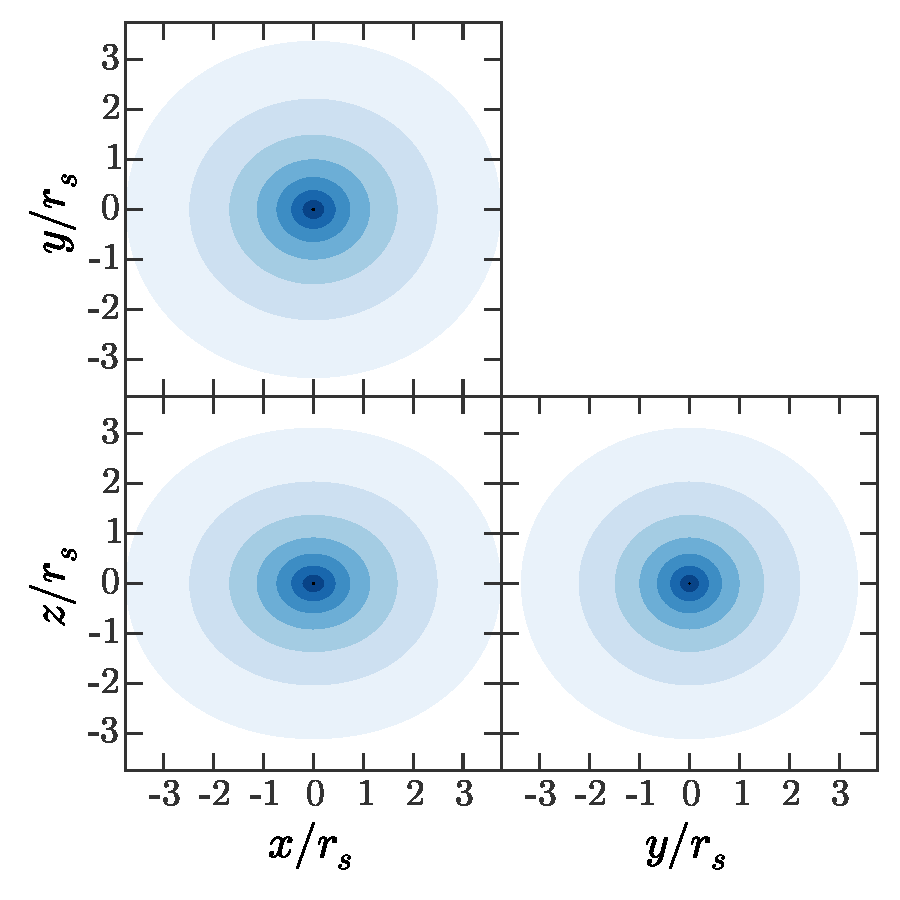
\includegraphics[width=\textwidth]{figures/potential.pdf}
\caption{Equipotential contours for the triaxial NFW potential considered in this work. There are eight contour levels evenly spaced and linear in the value of the potential. } \label{fig:potential}
\end{center}
\end{figure*}

% Figure 2
\begin{figure*}[p]
\begin{center}
\includegraphics[width=\textwidth]{figures/lyap-orbits.pdf}
\caption{ FTMLE (Equation~\ref{eq:ftmle}) computed over YYYY orbital periods for the stream-fanning Palomar 5 orbit of \cite{pearson15}. The FTMLE saturates to the Lyapunov exponent in the shaded region and is estimated to be $\lambda_{\rm max} \approx XXX \, {\rm Gyr}^{-1}$, corresponding to a Lyapunov time of $t_\lambda \approx XX \, {Gyr}$. Over-plotted on both panels are lines (dashed, blue) that show $t^{-0.9}$ behavior.} \label{fig:pal5}
\end{center}
\end{figure*}

% Figure 3
\begin{figure*}[p]
\begin{center}
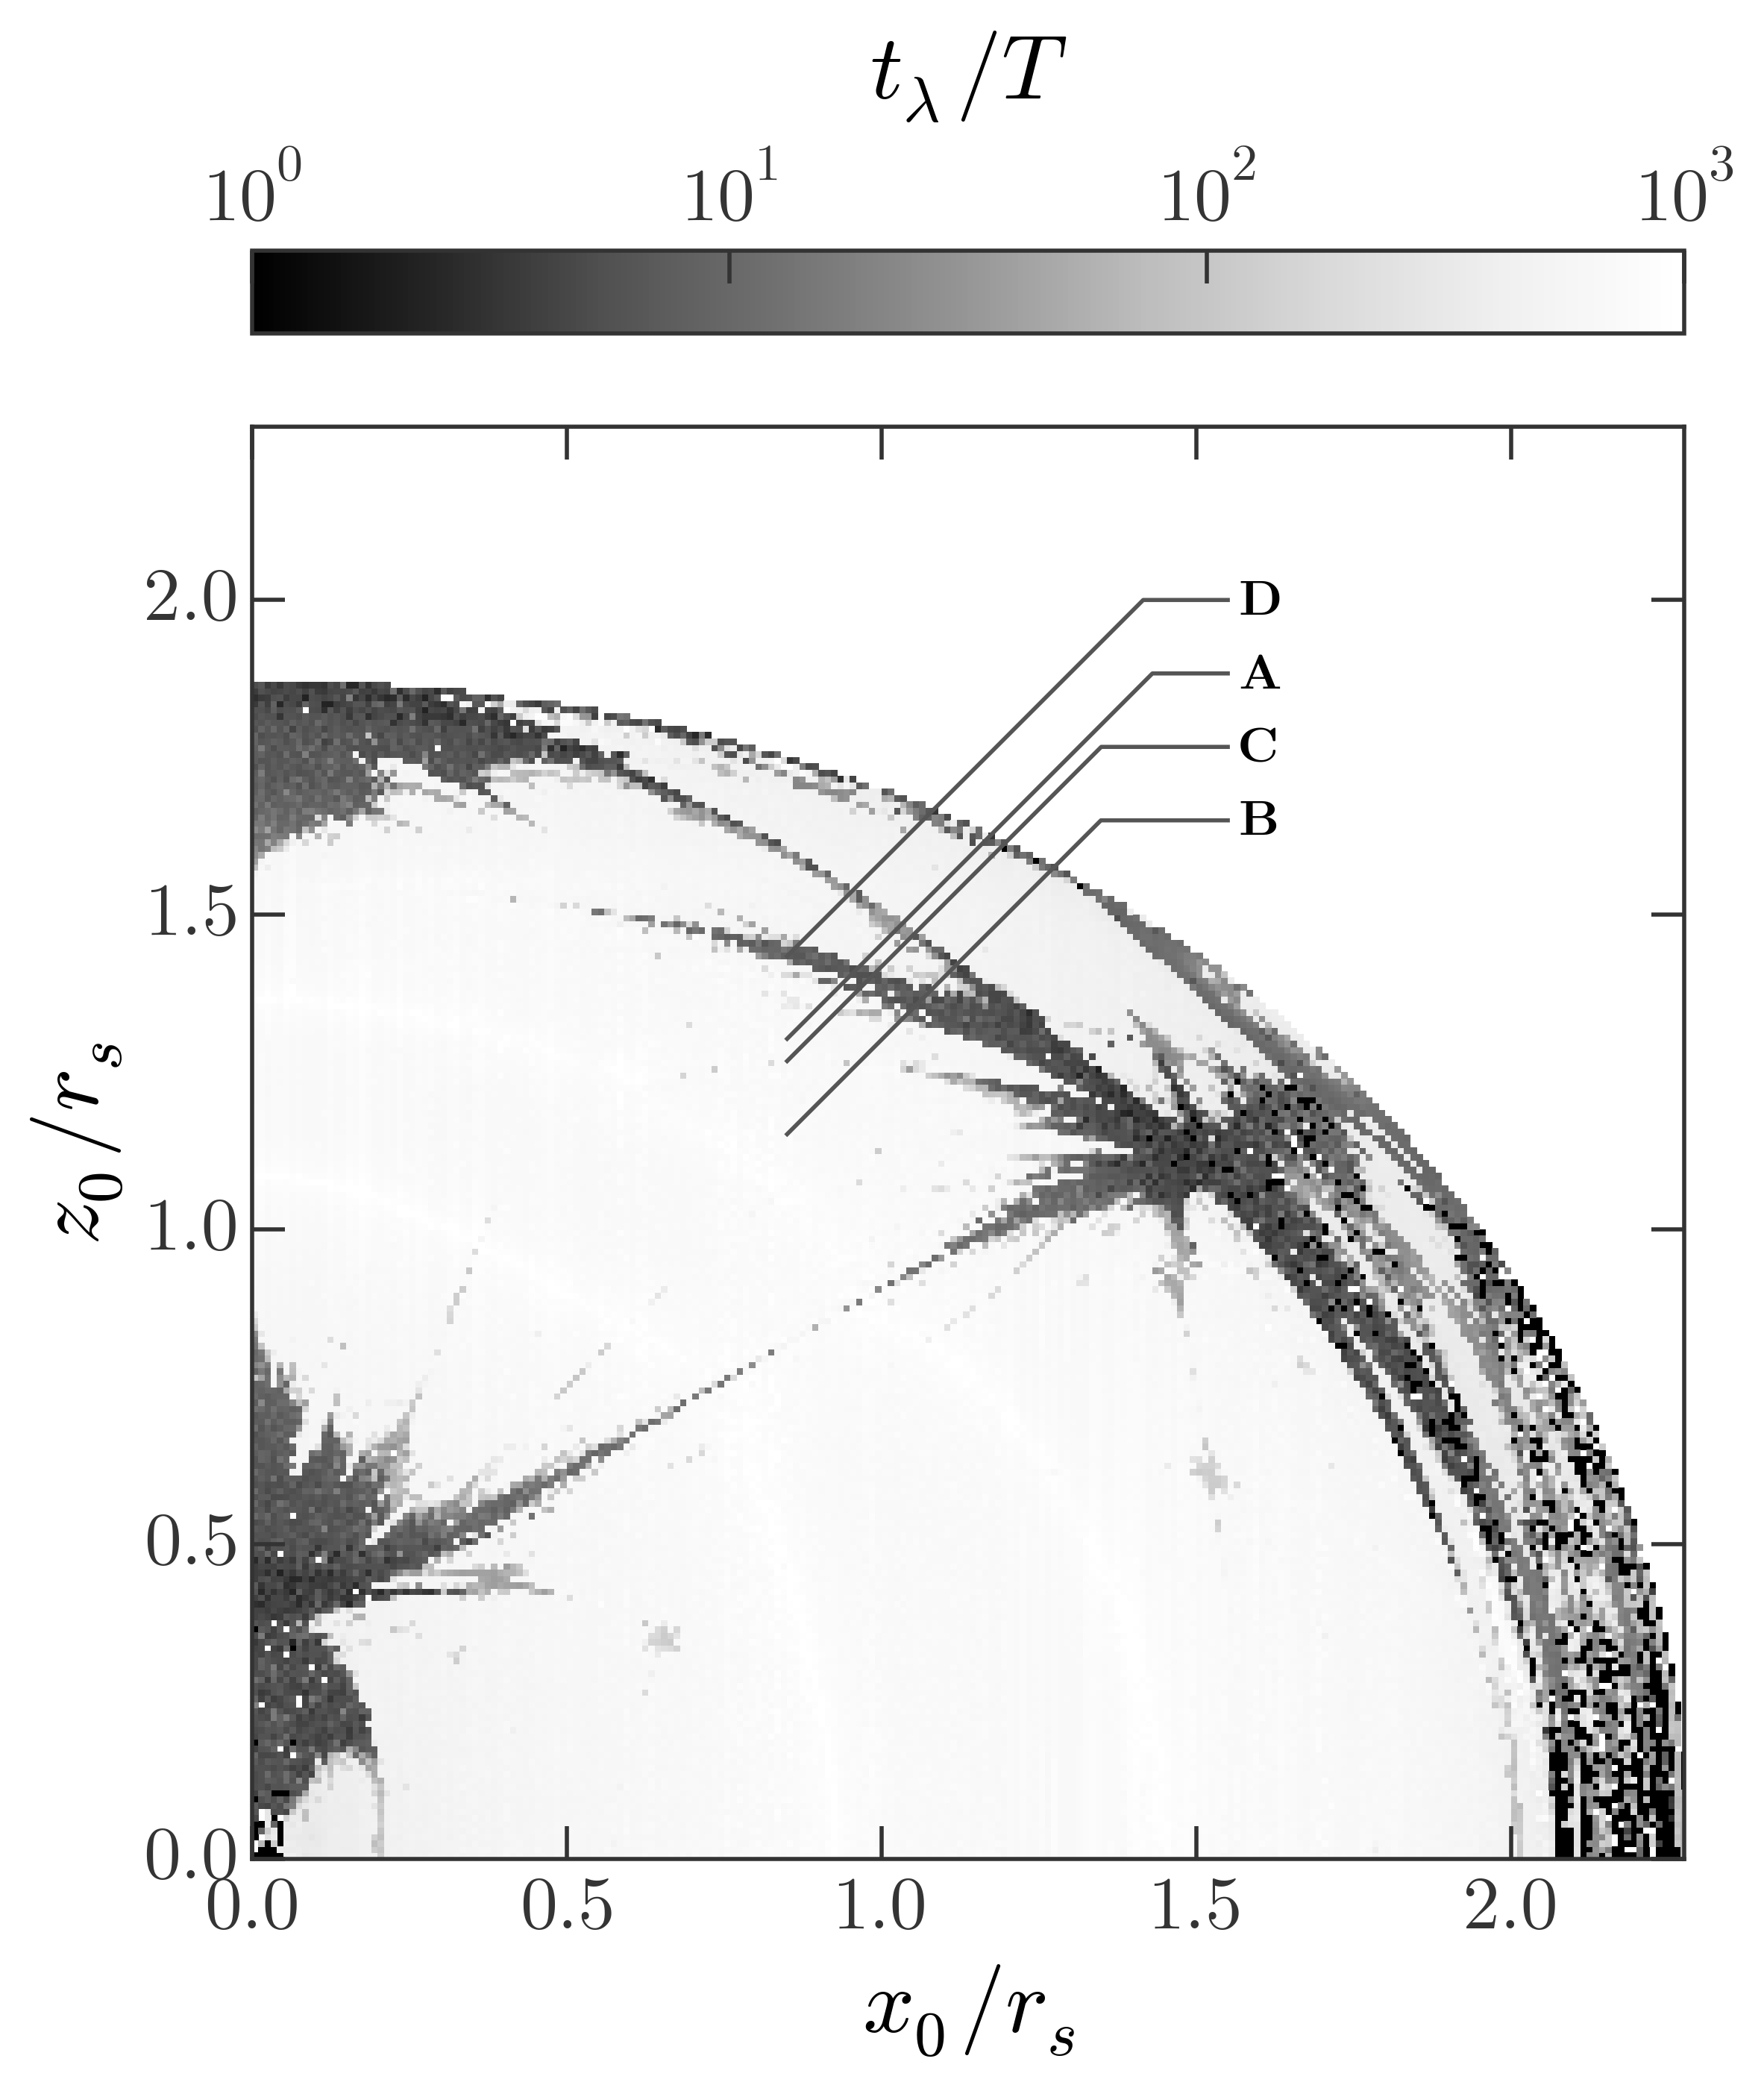
\includegraphics[width=\textwidth]{figures/lyap_map.png}
\caption{  } \label{fig:lyapmap} 
\end{center}
\end{figure*}

% Figure 4
\begin{figure*}[p]
\begin{center}
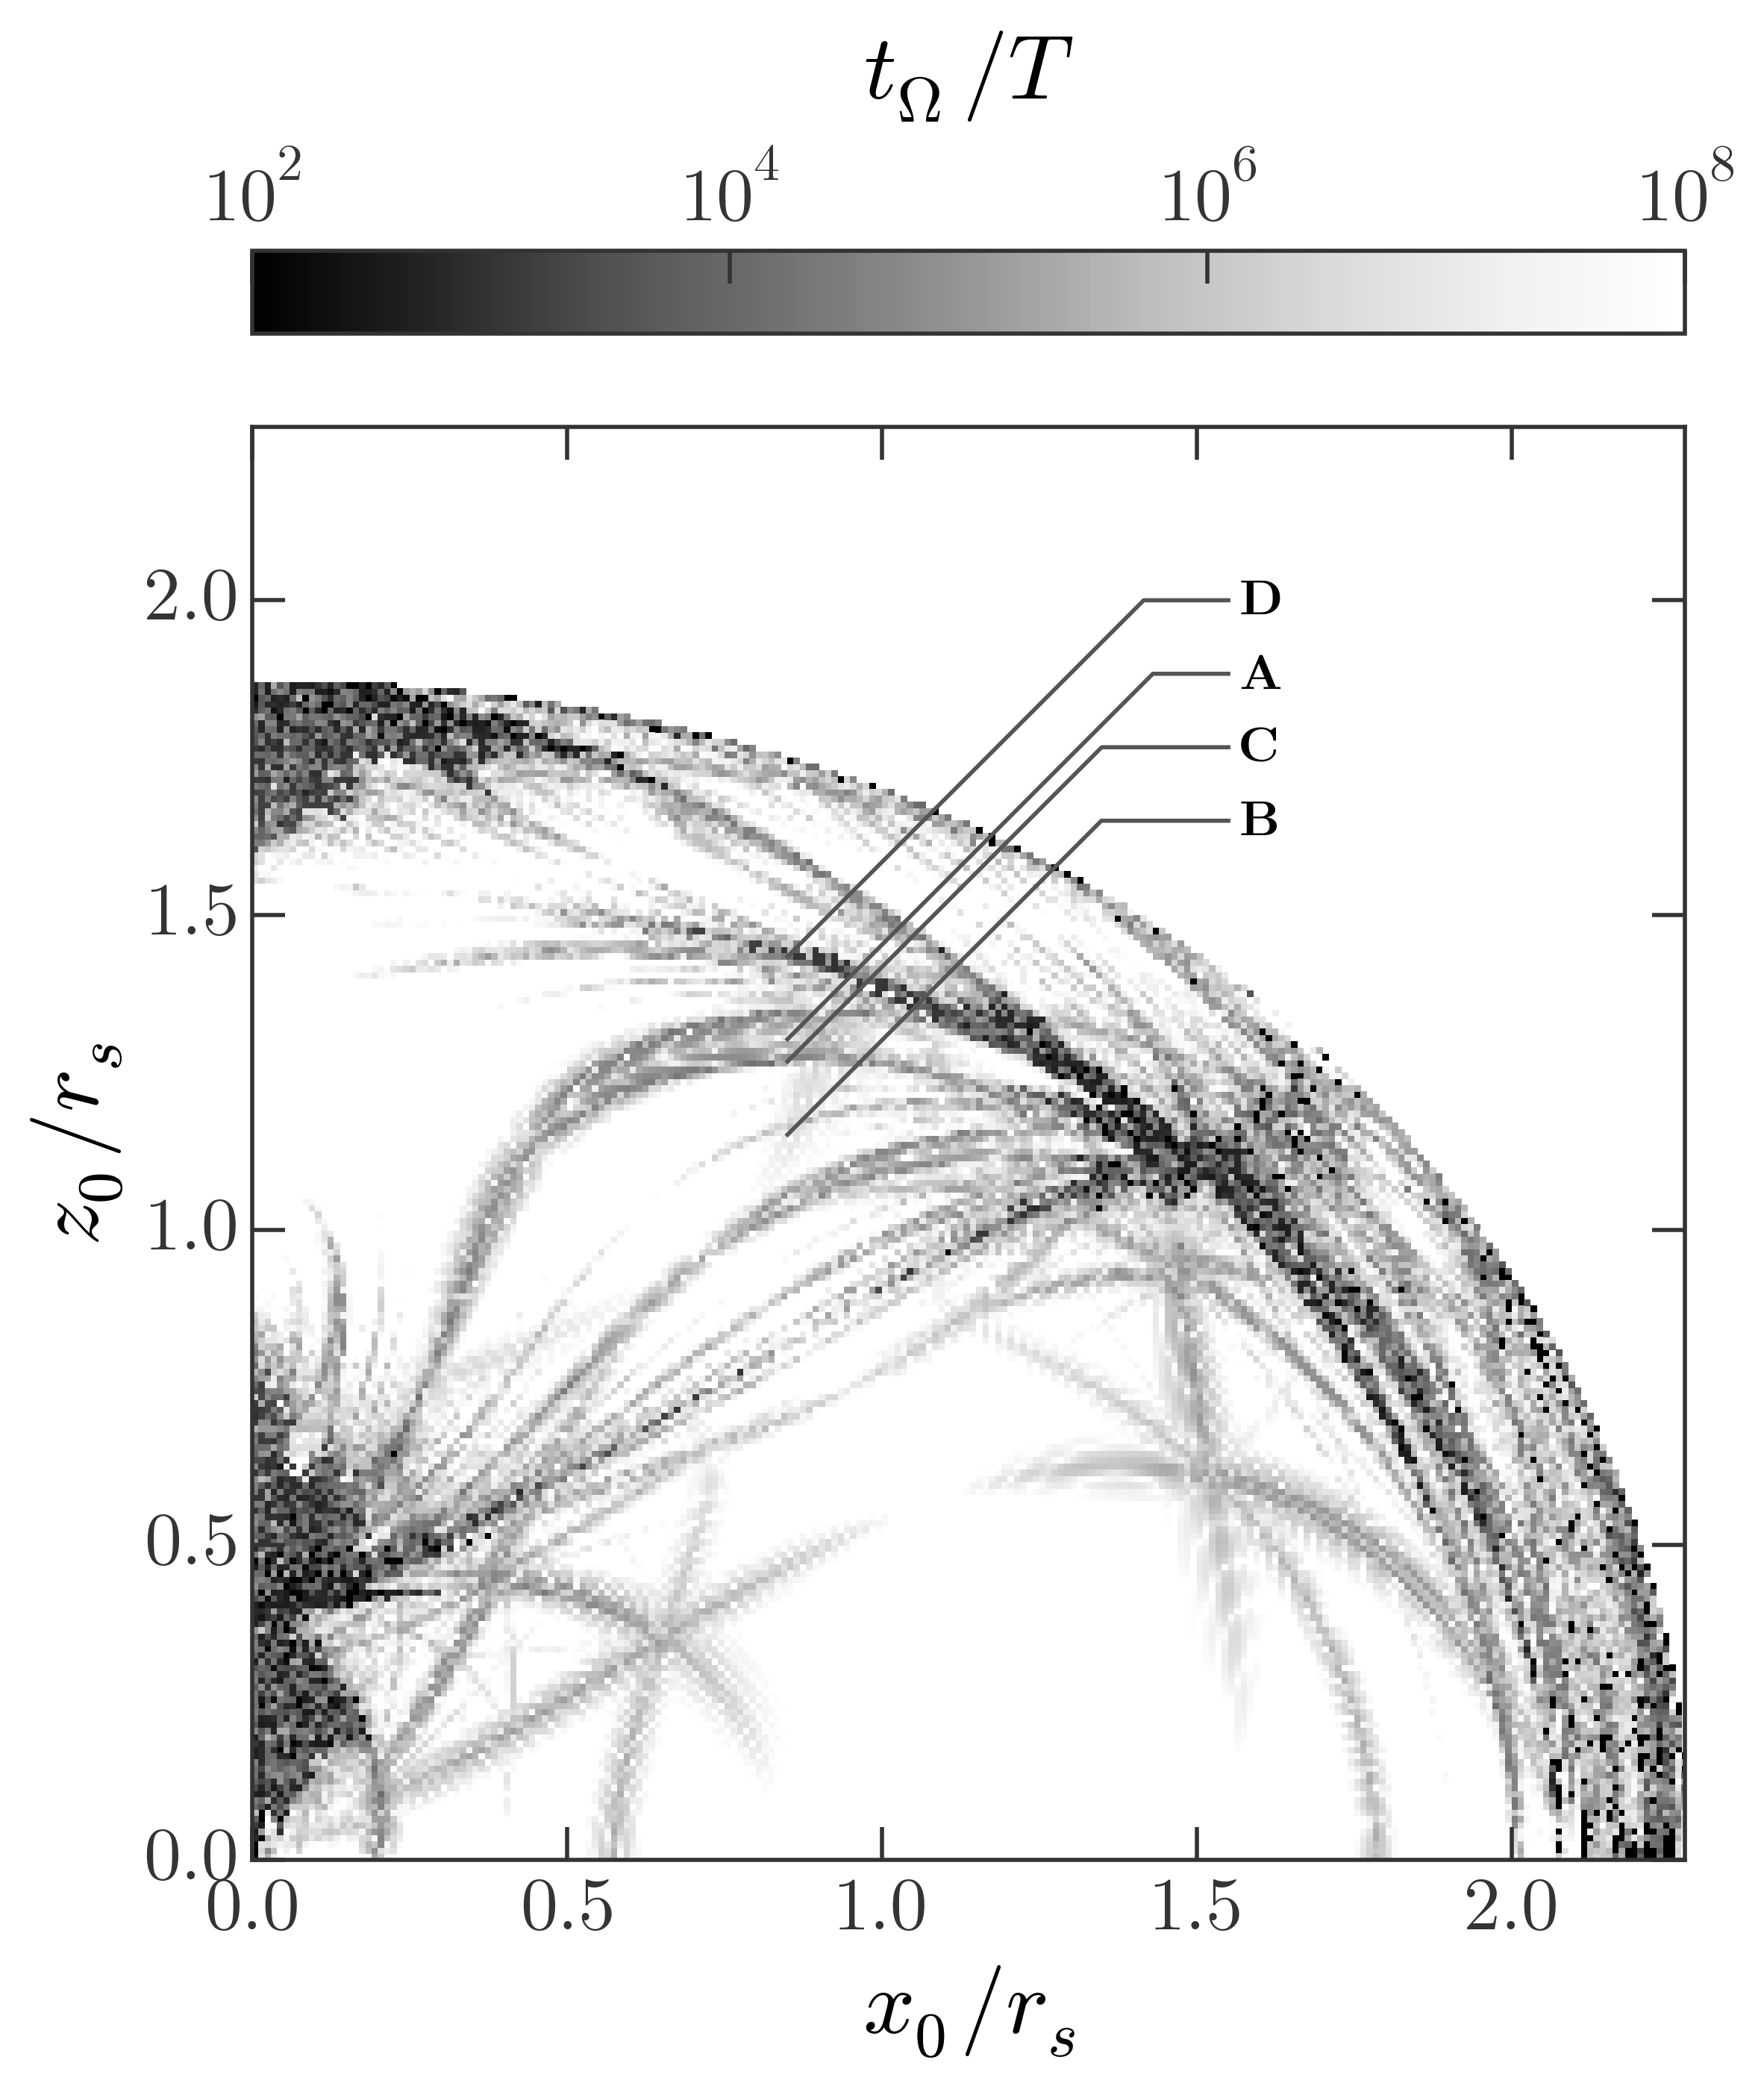
\includegraphics[width=\textwidth]{figures/fdiff_map.png}
\caption{This is really just a placeholder that shows what I want to show here...} \label{fig:freqdiff}
\end{center}
\end{figure*}

% Figure 5
\begin{figure*}[p]
\begin{center}
%\includegraphics[width=\textwidth]{figures/lyap_vs_fdiff.png}
\caption{This is really just a placeholder that shows what I want to show here...} \label{fig:lyapvfreqdiff}
\end{center}
\end{figure*}

% Figure 6
\begin{figure*}[p]
\begin{center}
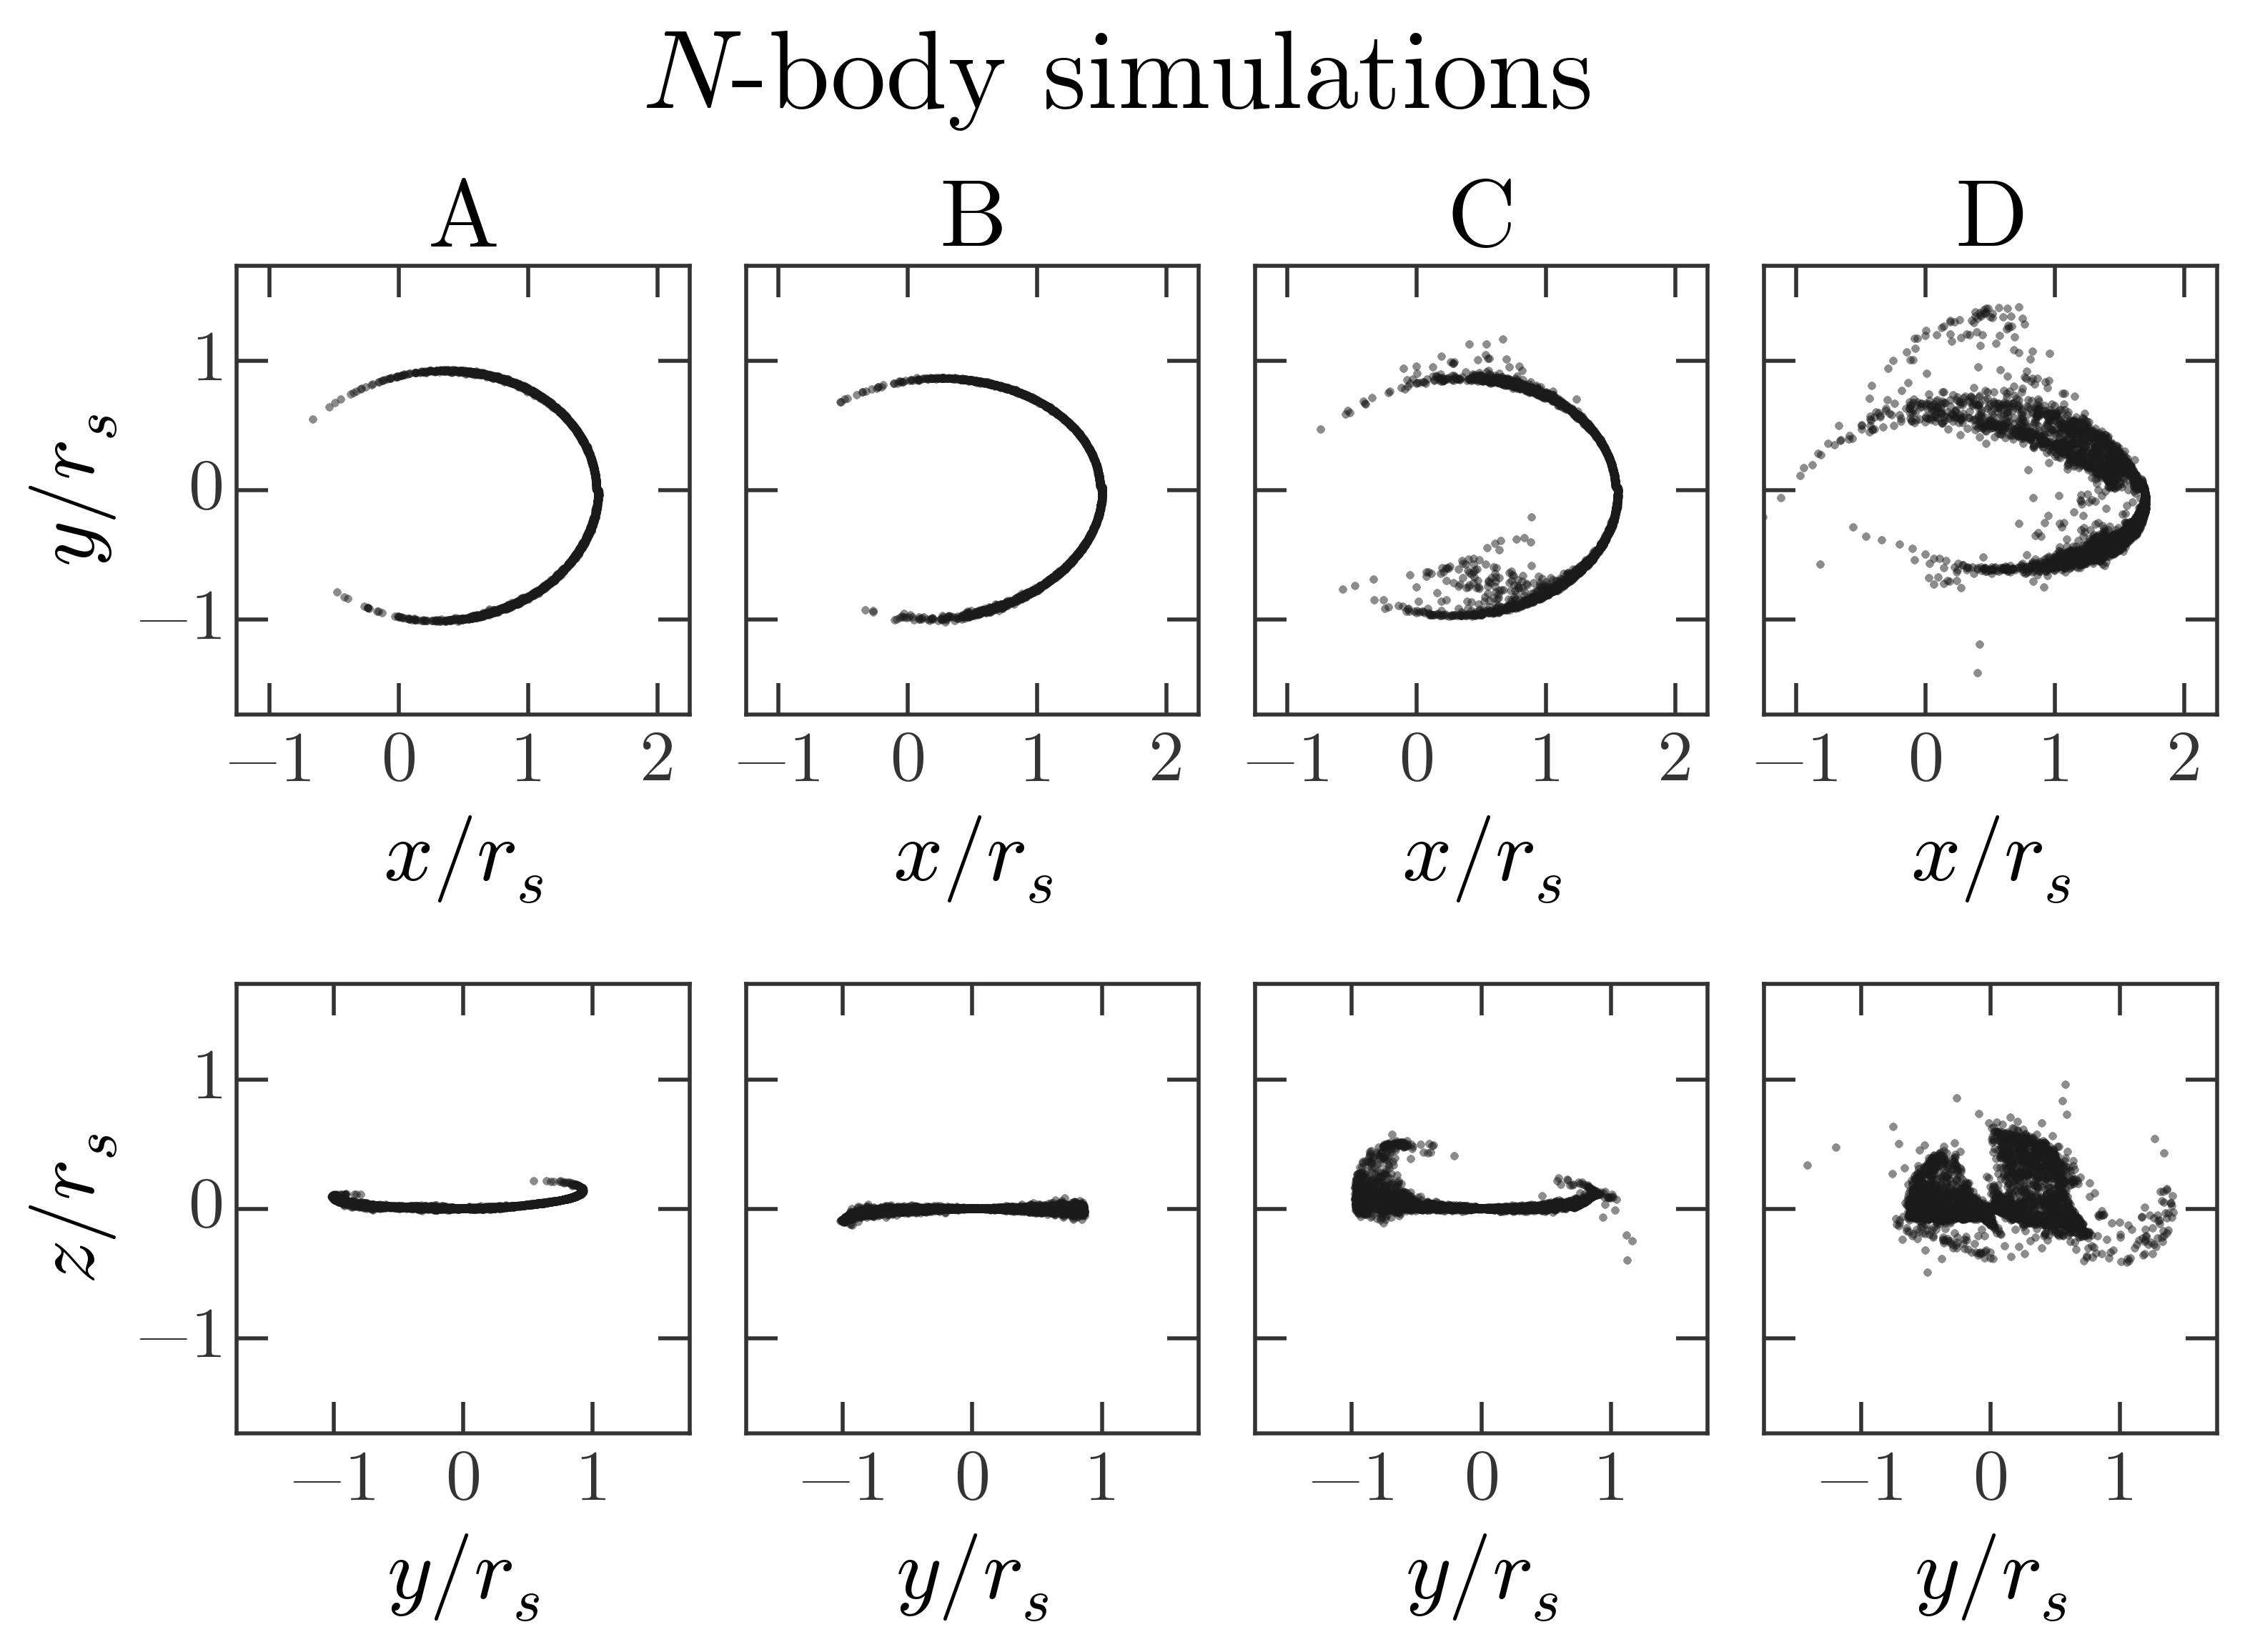
\includegraphics[width=\textwidth]{figures/nbody.png}
\caption{This is really just a placeholder that shows what I want to show here...} \label{fig:nbodysims}
\end{center}
\end{figure*}


\end{document}
